\documentclass{beamer}
\usepackage[T1]{fontenc}
\usepackage[utf8]{inputenc}
\usepackage{graphicx}
\usepackage[normalem]{ulem}
\usepackage{xmpmulti}
% \usepackage[dvipsnames]{xcolor}

\newcommand{\emphh}[1]{\textcolor{blue}{\emph{#1}}}
\newcommand{\hilite}[1]{\emphh{#1}}
\title{Connected Dominating Sets in \newline (Surface) Triangulations}

\newcommand{\verteq}{\rotatebox{90}{$\equiv$}}

\author{}
\author{%
  Prosenjit~Bose \and
  Vida~Dujmović \and
  Hussein~Houdrouge \and
  Pat~Morin \and
  Saeed~Odak}
\date{}

\setbeameroption{hide notes} % Only slides
%\setbeameroption{show only notes} % Only notes
% \setbeameroption{show notes on second screen=right} % Both


% \DeclareMathOperator{\tw}{tw}
% \DeclareMathOperator{\td}{td}
% \DeclareMathOperator{\wcol}{wcol}
% \DeclareMathOperator{\lvr}{\chi_{\ell-\mathrm{vr}}}
% \DeclareMathOperator{\pcn}{\chi_{p}}

\begin{document}

\begin{frame}
  % \begin{center}
    \maketitle
  % \end{center}
\end{frame}

\begin{frame}
  \frametitle{Outline}

  \begin{itemize}
    % \item Two applications
    \item Basics
    \item (Connected) dominating sets
    \item Connections with other problems
    \item Analysis of naïve greedy strategy
    \item Analysis of best strategy (so far)
    \item Directions for future work
  \end{itemize}
\end{frame}

% \begin{frame}
%   \frametitle{SEFENOMAP}
%   \uncover<3->{\textbf{Theorem (Angelini, Evans, Frati, and Gudmundsson 2016):}  If $|G_1|=n$ and $|G_2|\le n/2$ then SEFENOMAP has a solution.}
%
%   \begin{center}
%     \begin{tabular}{cc}
%     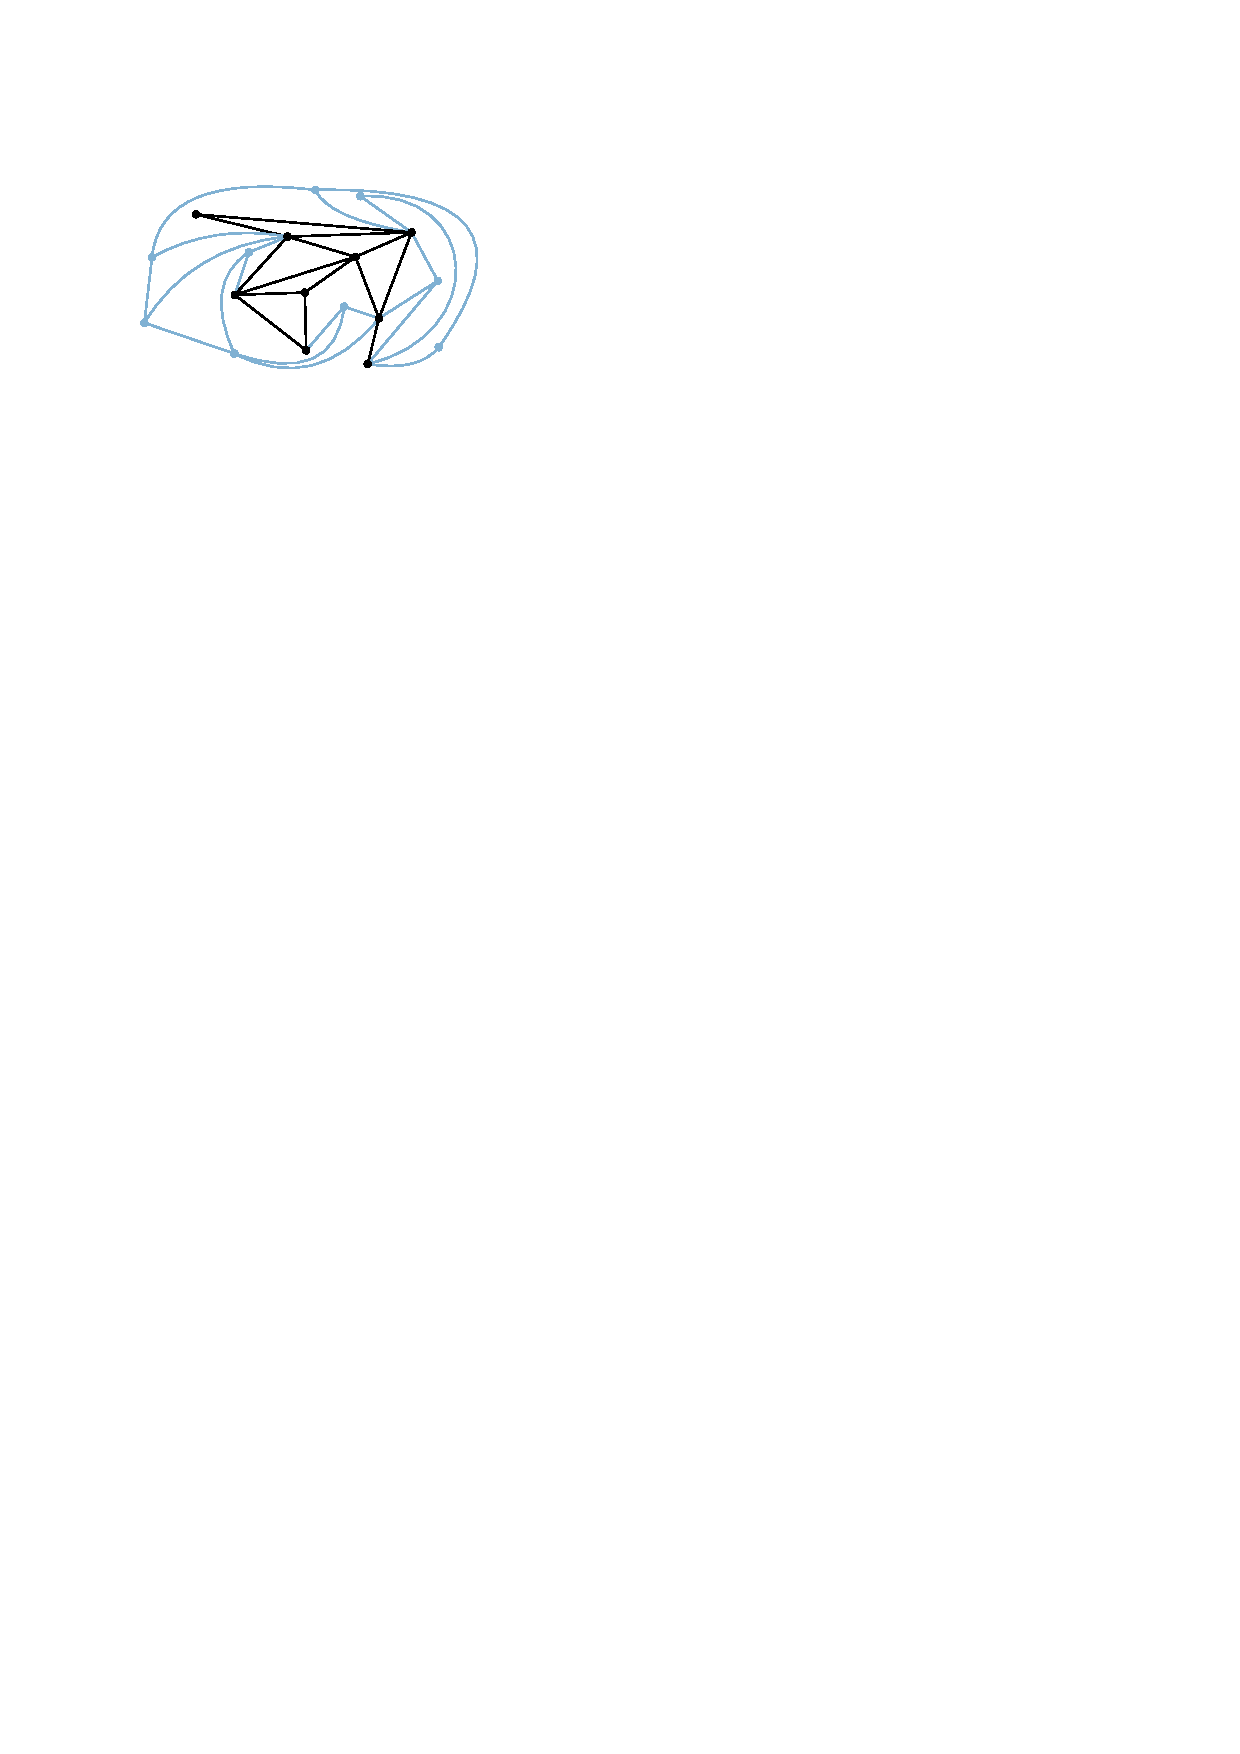
\includegraphics[page=1,scale=.8]{figs/sefenomap} & \includegraphics[page=2,scale=.8]{figs/sefenomap} \\
%     $G_1$ & $G_2$
%   \end{tabular}
%     \uncover<2->{\includegraphics[page=3,scale=.8]{figs/sefenomap}}
%   \end{center}
%   \uncover<4>{\textbf{Solution:} Find induced outerplane graph $G_1[S]$ with $|S|=|V(G_2)|$}
% \end{frame}
%
% \begin{frame}
%   \frametitle{Free Sets}
%
%   $S\subseteq V(G)$ is a \emphh{free set} if, for every $|S|$-point set $P$, $G$ has a \emphh{straight-line} non-crossing drawing with all vertices in $S$ mapped to points in $P$.\\[1em]
%
%   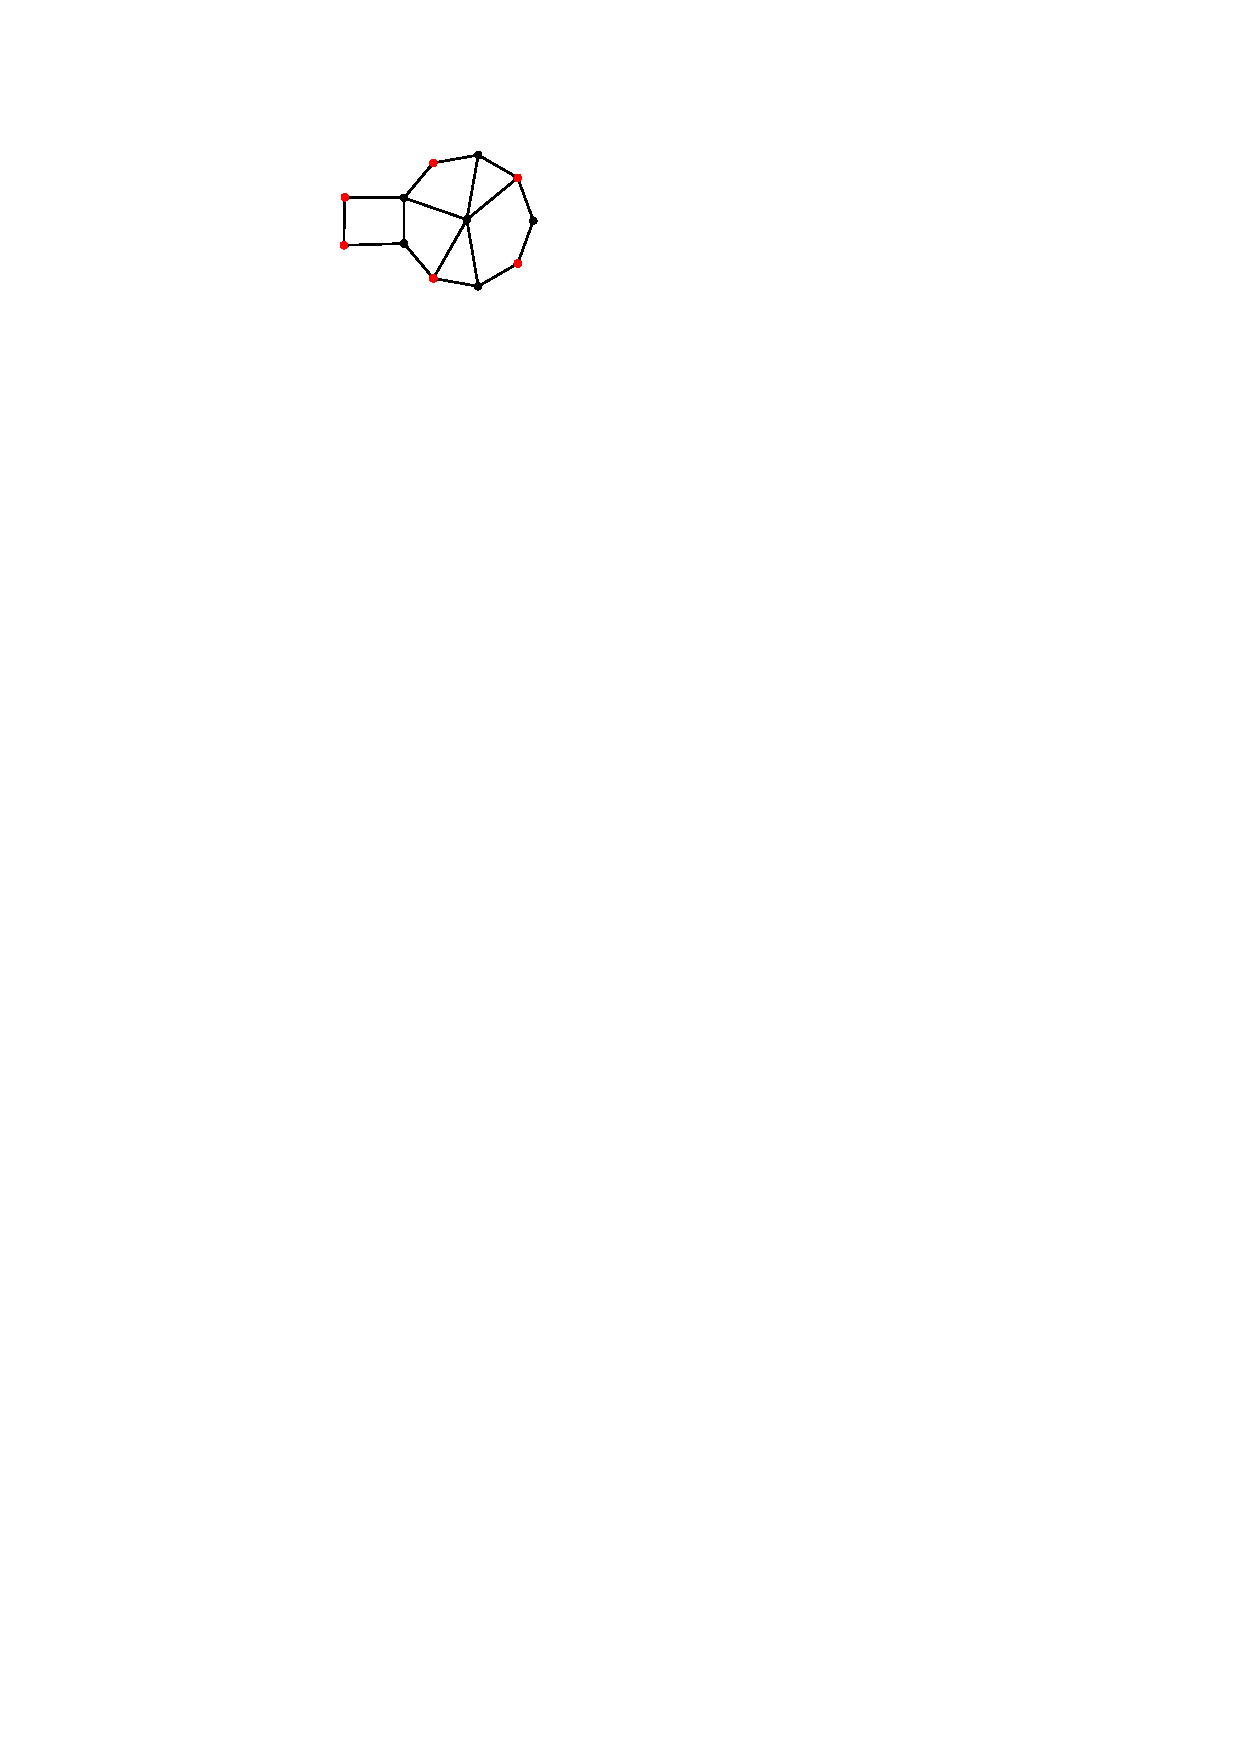
\includegraphics[page=1]{figs/universal}%
%   \only<2>{\includegraphics[page=2]{figs/universal}}%
%   \only<3>{\includegraphics[page=3]{figs/universal}}%
%   \only<4>{\includegraphics[page=4]{figs/universal}}%
%   \only<5>{\includegraphics[page=5]{figs/universal}}%
%   \only<6>{\includegraphics[page=6]{figs/universal}}%
%   \only<7->{\includegraphics[page=7]{figs/universal}}%
%
%
%   \uncover<8->{\textbf{Theorem (Bose-Da~Lozzo-Dujmović-Frati-Hurtado-Langerman-Mchedlidze--M-Roselli-Rote-Wood 2009--2021):} Every $n$-vertex planar graph $G$ has a free set of size $\Omega(\sqrt{n})$.\\[1em]
%
%   \textbf{Theorem (Ravsky-Verbistky 2011):}  There exists $n$-vertex planar $G$ with no free set of size $\Omega(n^{0.98583})$.}
% \end{frame}
%
% \begin{frame}
%   \frametitle{Free Sets, Collinear Sets, and Proper Good Curves}
%   % \uncover<2->{$S$ is a free-set iff and only if $S$ is contained in a \emphh{proper good curve}}
%   \begin{center}
%     \includegraphics[page=2,scale=0.8]{figs/1-proper}
%   \end{center}
%   % \uncover<2->{$S\subseteq V(G)$ is a \emphh{one-bend free set} if, for every $|S|$-point set $P$, $G$ has a \emphh{one-bend} non-crossing drawing with all vertices in $S$ mapped to points in $P$.}
% \end{frame}
%
% \begin{frame}
%   \frametitle{One-Bend Free Sets}
%
%   $S\subseteq V(G)$ is a \emphh{one-bend free set} if, for every $|S|$-point set $P$, $G$ has a \emphh{one-bend} non-crossing drawing with all vertices in $S$ mapped to points in $P$.\\[1em]
%   % $S\subseteq V(G)$ is a \emphh{free set} if, for every $|S|$-point set $P$, $G$ has a \emphh{straight-line} non-crossing drawing with all vertices in $S$ mapped to points in $P$.\\[1em]
%
%   % \textbf{Theorem (Here):} Every $n$-vertex planar graph $G$ has a one-bend free set of size at least $11n/21$.\\[2em]
%
%   \textbf{Theorem (Goldner-Harary):}  There exists $n$-vertex planar $G$ with no free set of size greater than $10n/11$.\\[1em]
%
%   \uncover<2->{\textbf{Observation:} $S\subseteq V(G)$ is a one-bend free set iff $S$ is a free set in a $1$-subdvision of $G$}
%
%   \only<1-2>{\includegraphics[page=9]{figs/proper_good}}%
%   \only<3>{\includegraphics[page=7]{figs/proper_good}}%
%   \only<4->{\includegraphics[page=8]{figs/proper_good}}%
% \end{frame}

\begin{frame}
  \frametitle{Basics}

  \begin{itemize}
    \item Graph, adjacency, neighbourhood, induced subgraphs
    \item Plane graph
    \item Triangulation
    \item (Generalized) near-triangulation
    \item Outerplanar triangulation
  \end{itemize}
\end{frame}

\begin{frame}
  \frametitle{(Connected) Dominating Sets}

  \begin{itemize}[<+->]
    \item $X\subseteq V(G)$ is a \emphh{dominating set} of $G$ if $N[X]=V(G)$
    \begin{center}
      \only<1>{\includegraphics[page=10]{figs/walkthrough}}%
      \only<2>{\includegraphics[page=11]{figs/walkthrough}}%
    \end{center}
    \item $X$ is \emphh{connected} if $G[X]$ is connected
  \end{itemize}
\end{frame}


\begin{frame}
  \frametitle{Connected Dominating Sets and Lush Spanning Trees}

  \begin{center}
    $X$ is a connected dominating set of $G$ \\[1em]
    $\Updownarrow$ \\[1em]
    $G$ has a spanning tree where vertices in $V(G)\setminus X$ are leaves.
    \only<1>{\includegraphics[page=11]{figs/walkthrough}}%
    \only<2>{\includegraphics[page=12]{figs/walkthrough}}%
    \only<3>{\includegraphics[page=9]{figs/walkthrough}}%
  \end{center}
\end{frame}

\begin{frame}
  \frametitle{Triangulations}

  \textbf{Theorem (Albertson, Berman, Hutchinson, and Thomassen 1990):}  Every triangulation has a \hilite{homemorphically irreducible} spanning tree.\\[2em]

  \uncover<2->{\textbf{Corollary:} Every $n$-vertex triangulation has a spanning tree with at least $n/2$ leaves.\\[2em]}

  \uncover<3->{\textbf{Corollary:} Every $n$-vertex triangulation has a connected dominating set of size at least $n/2$.}
\end{frame}

\begin{frame}
  \frametitle{Induced Outerplane Graphs}

  \begin{center}
    \only<1>{\includegraphics[page=13]{figs/walkthrough}}%
    \only<2->{\includegraphics[page=14]{figs/walkthrough}}%
  \end{center}

  \uncover<2->{\textbf{Observation:} If $X$ is a connected dominating set then $G-X$ is an induced outerplane graph with $n-|X|$ vertices.}\\[2em]

  % \uncover<3->{Better solution to SEFENOMAP if $|X|< n/2$}
\end{frame}

% \begin{frame}
%   \frametitle{$2$-Proper Good Curves}
%
%   \begin{center}
%     \only<1>{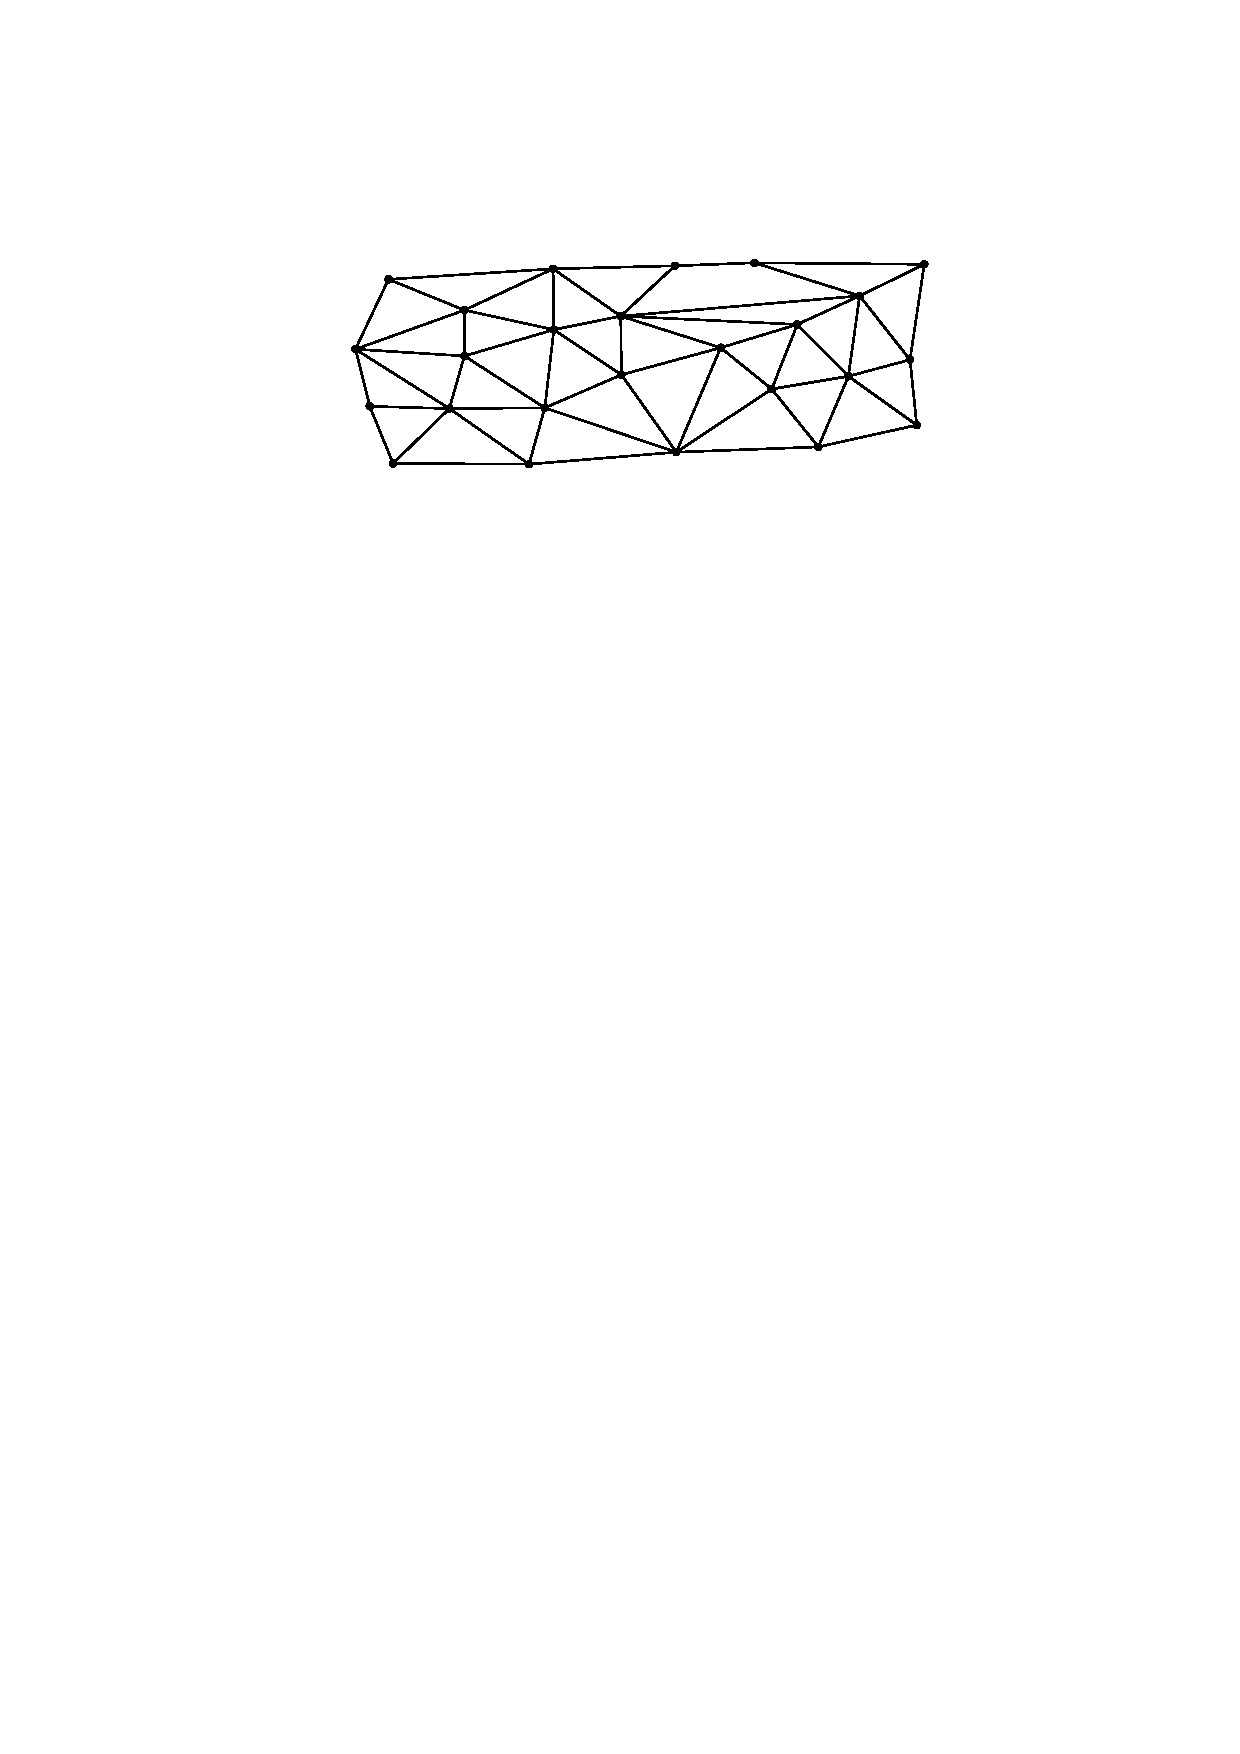
\includegraphics[page=1]{figs/proper_good}}%
%     \only<2>{\includegraphics[page=2]{figs/proper_good}}%
%     \only<3>{\includegraphics[page=3]{figs/proper_good}}%
%     \only<4>{\includegraphics[page=4]{figs/proper_good}}%
%     \only<5>{\includegraphics[page=5]{figs/proper_good}}%
%     \only<6->{\includegraphics[page=6]{figs/proper_good}}%
%     % \only<7>{\includegraphics[page=7]{figs/proper_good}}%
%     % \only<8>{\includegraphics[page=8]{figs/proper_good}}%
%   \end{center}
%
%   \uncover<7->{\textbf{Observation:} If $X$ is a connected dominating set then $V(G)\setminus X$ is a one-bend free set.}
% \end{frame}


\begin{frame}
  \frametitle{The Benchmark: $n/3$}

  \begin{center}
    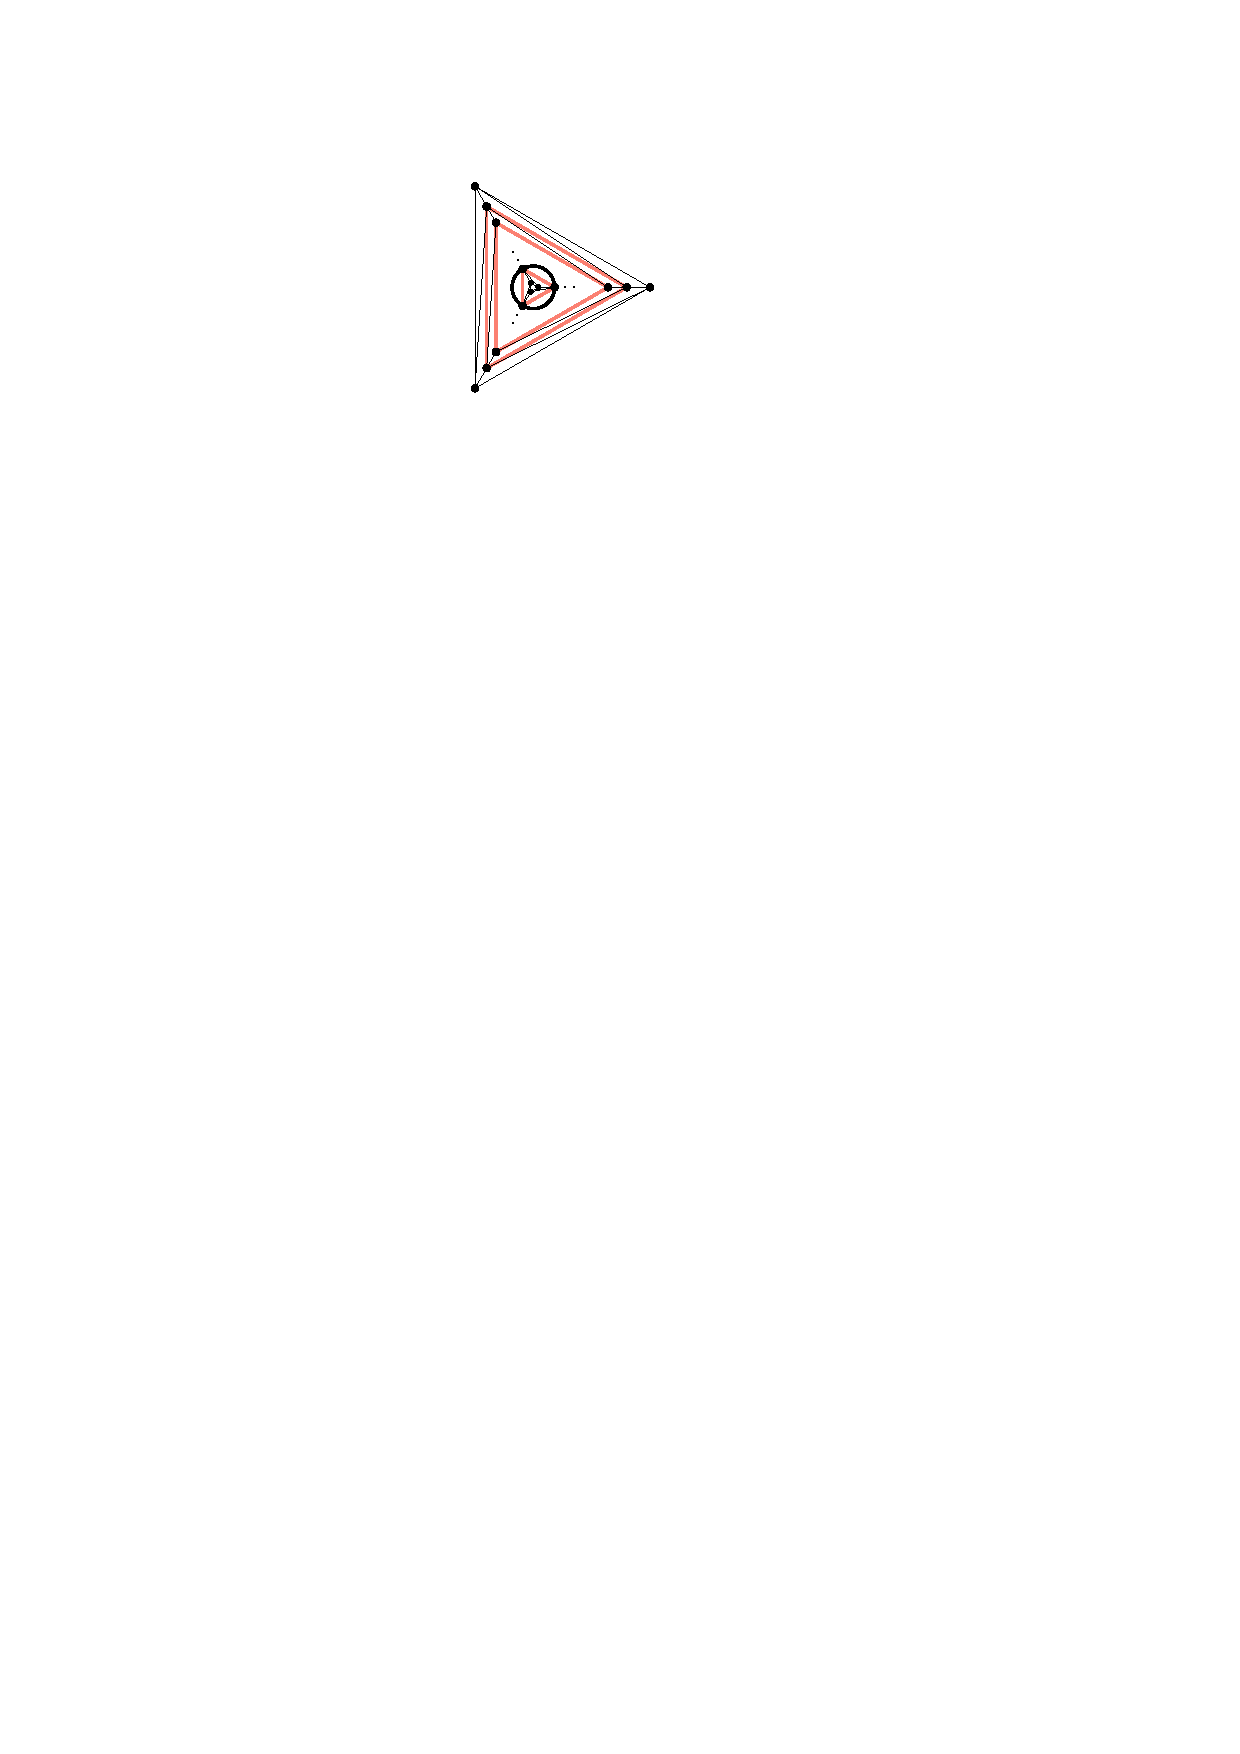
\includegraphics[height=.7\textheight]{figs/nover3}
  \end{center}
\end{frame}


% \begin{frame}
%   \frametitle{Proper Good Curves}
%
%   Free sets correspond to vertices on a \emphh{proper good curves}:
%
%   One-bend free sets correspond to vertices on a \emphh{$2$-proper good curve}.
%
% \end{frame}

\begin{frame}
  \frametitle{Main Result}

  \uncover<+->{\textbf{Theorem:}  Every $n$-vertex triangulation $G$ has a connected dominating set of size at most $10n/21=\overline{0.476190}n$.}\\[2em]

  \uncover<+->{\textbf{Corollary:}  Every $n$-vertex triangulation $G$ has a spanning tree with at least $11n/21=\overline{0.523809}n$ leaves.}\\[2em]

  \uncover<+->{\textbf{Corollary:}  Every $n$-vertex triangulation $G$ has an induced outerplane graph $G[Y]$ with at least $11n/21=\overline{0.523809}n$ vertices.}\\[2em]

  % \uncover<+->{\textbf{Corollary:}  A bound of $11n/21$ for SEFENOMAP.}\\[2em]
  %
  % \uncover<+->{\textbf{Corollary:}  Every $n$-vertex planar graph has a one-bend free set of size $11n/21$.}
\end{frame}

\begin{frame}
  \frametitle{NaïveGreedy Strategy}

  \begin{tabular}{p{.6\textwidth}c}

    $\textsc{NaïveGreedy}(G)$:\newline
    $X\gets\{v_0\}$ \newline
    Repeat until $N[X]=V(G)$: \newline
    --- Let $v\in N(X)$ maximize $|N(v)\setminus N(X)|$ \newline
    --- Set $X\gets X\cup\{v\}$
    &
    \raisebox{-\height}{%
      \only<1>{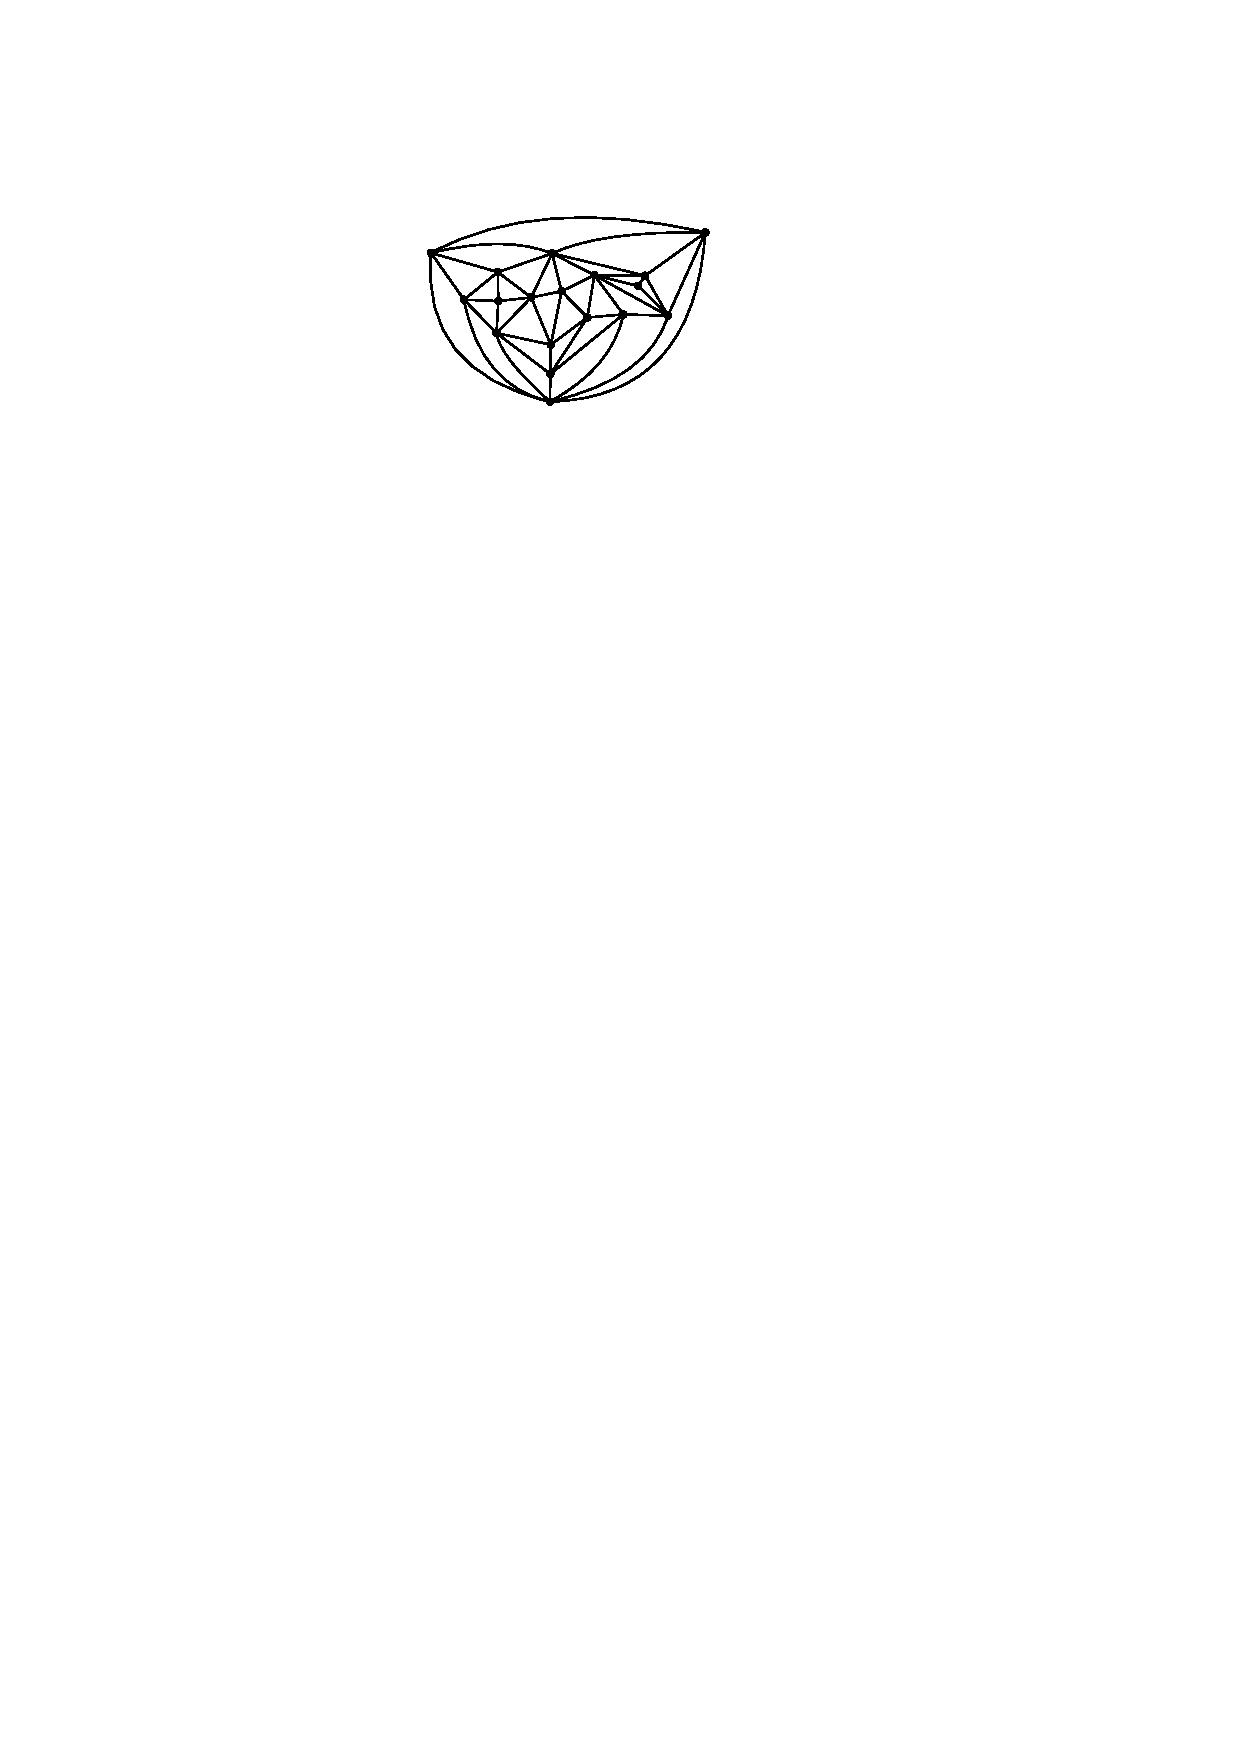
\includegraphics[width=.4\textwidth,page=1]{figs/walkthrough}}%
      \only<2>{\includegraphics[width=.4\textwidth,page=2]{figs/walkthrough}}%
      \only<3>{\includegraphics[width=.4\textwidth,page=3]{figs/walkthrough}}%
      \only<4>{\includegraphics[width=.4\textwidth,page=4]{figs/walkthrough}}%
      \only<5>{\includegraphics[width=.4\textwidth,page=5]{figs/walkthrough}}%
      \only<6-7>{\includegraphics[width=.4\textwidth,page=6]{figs/walkthrough}}%
      \only<8>{\includegraphics[width=.4\textwidth,page=7]{figs/walkthrough}}%
      \only<9>{\includegraphics[width=.4\textwidth,page=8]{figs/walkthrough}}%
      % \only<10>{\includegraphics[width=.4\textwidth,page=9]{figs/walkthrough}}%
    }
  \end{tabular}


  \begin{tabular}{p{.6\textwidth}c}
    \raggedright
    \uncover<4->{
    \textbf{Ideally:} $|N(v)\setminus N(X)|\ge c$ at each step \newline
    Would give $|X|\le n/c$\vspace{1em}
    }

    \uncover<6->{
    \textbf{Problem:} Impossible to guarantee $|N(v)\setminus N(X)|\ge 2$.\vspace{1em}
    }

    & \uncover<7->{\raisebox{-\height}{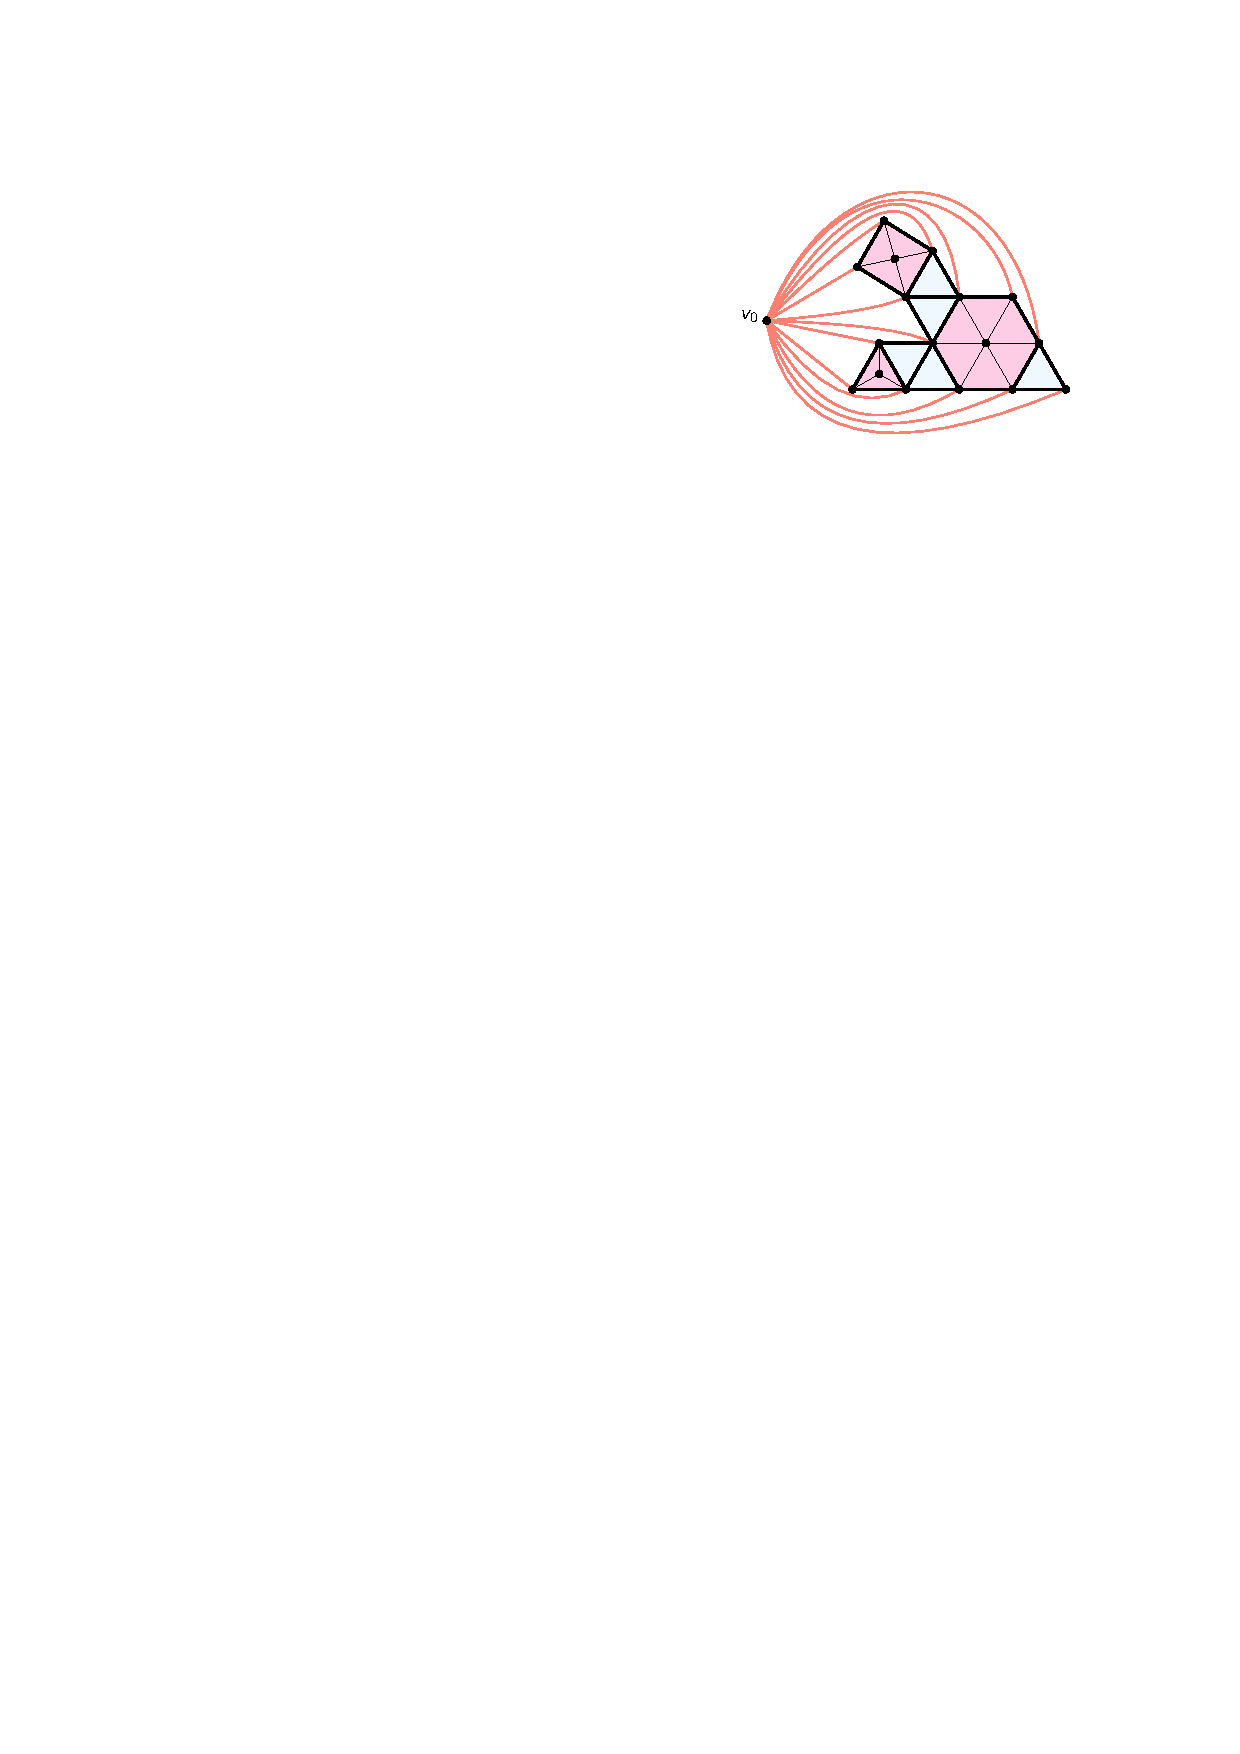
\includegraphics[width=.4\textwidth]{figs/noguarantee}}}
  \end{tabular}
\end{frame}


\begin{frame}
  \frametitle{$1$-Critical Graphs}

  All inner faces are triangles \newline
  All vertices have inner degree $\le 1$ \\[3em]

  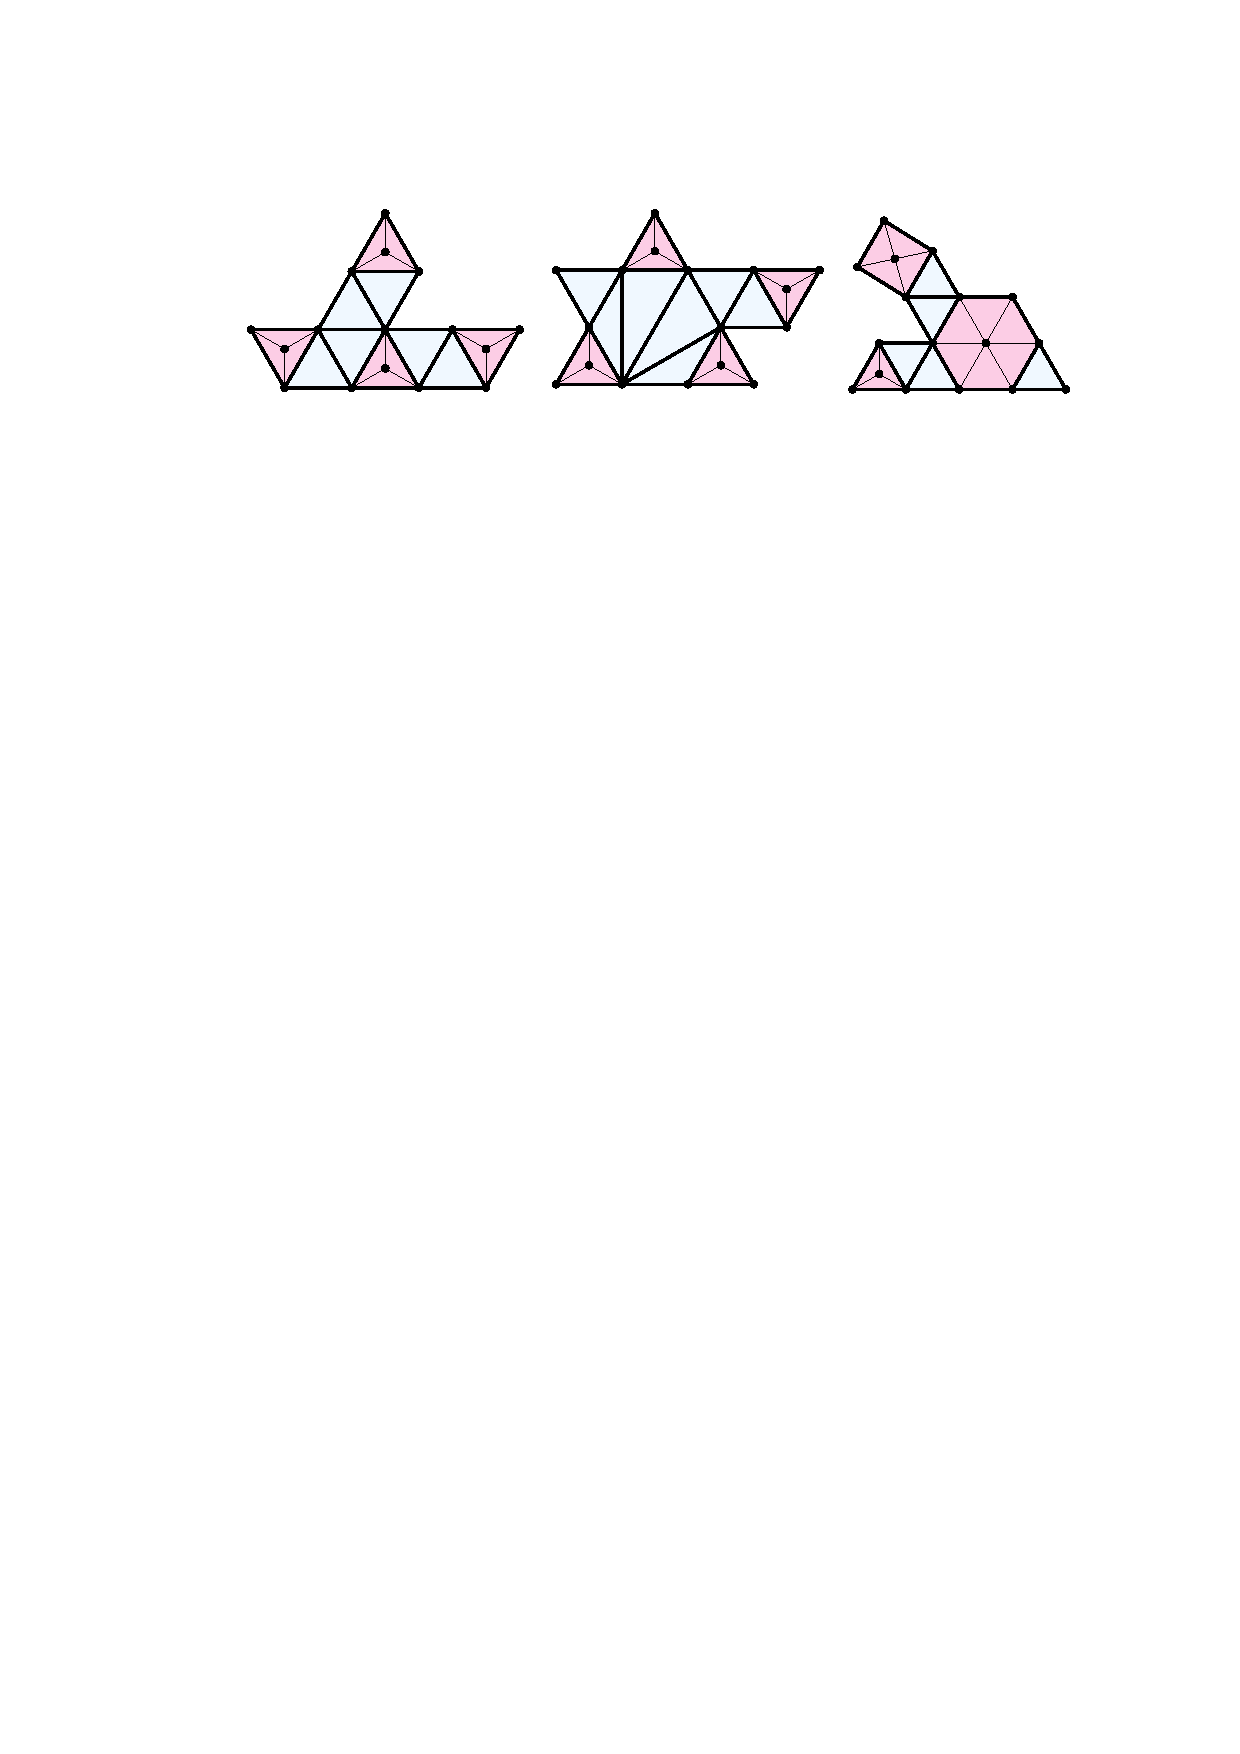
\includegraphics[width=.98\textwidth]{figs/critical}\\[3em]

  \textbf{Lemma:} $\text{\#inner vertices} \le \tfrac{1}{4}\text{\#vertices}$
\end{frame}

\begin{frame}
  \frametitle{A First Attempt}

  \textbf{Theorem:} $\textsc{NaïveGreedy}(G)$ produces a connected dominating set $X$ of size at most $4n/7$.\\[1em]

  \uncover<2->{
  \textit{Proof:} Takes vertices of inner-degree at least $2$ until $G-X$ is $1$-critical then takes $I:=V(G)-N[X]$ additional vertices.
  \begin{center}
    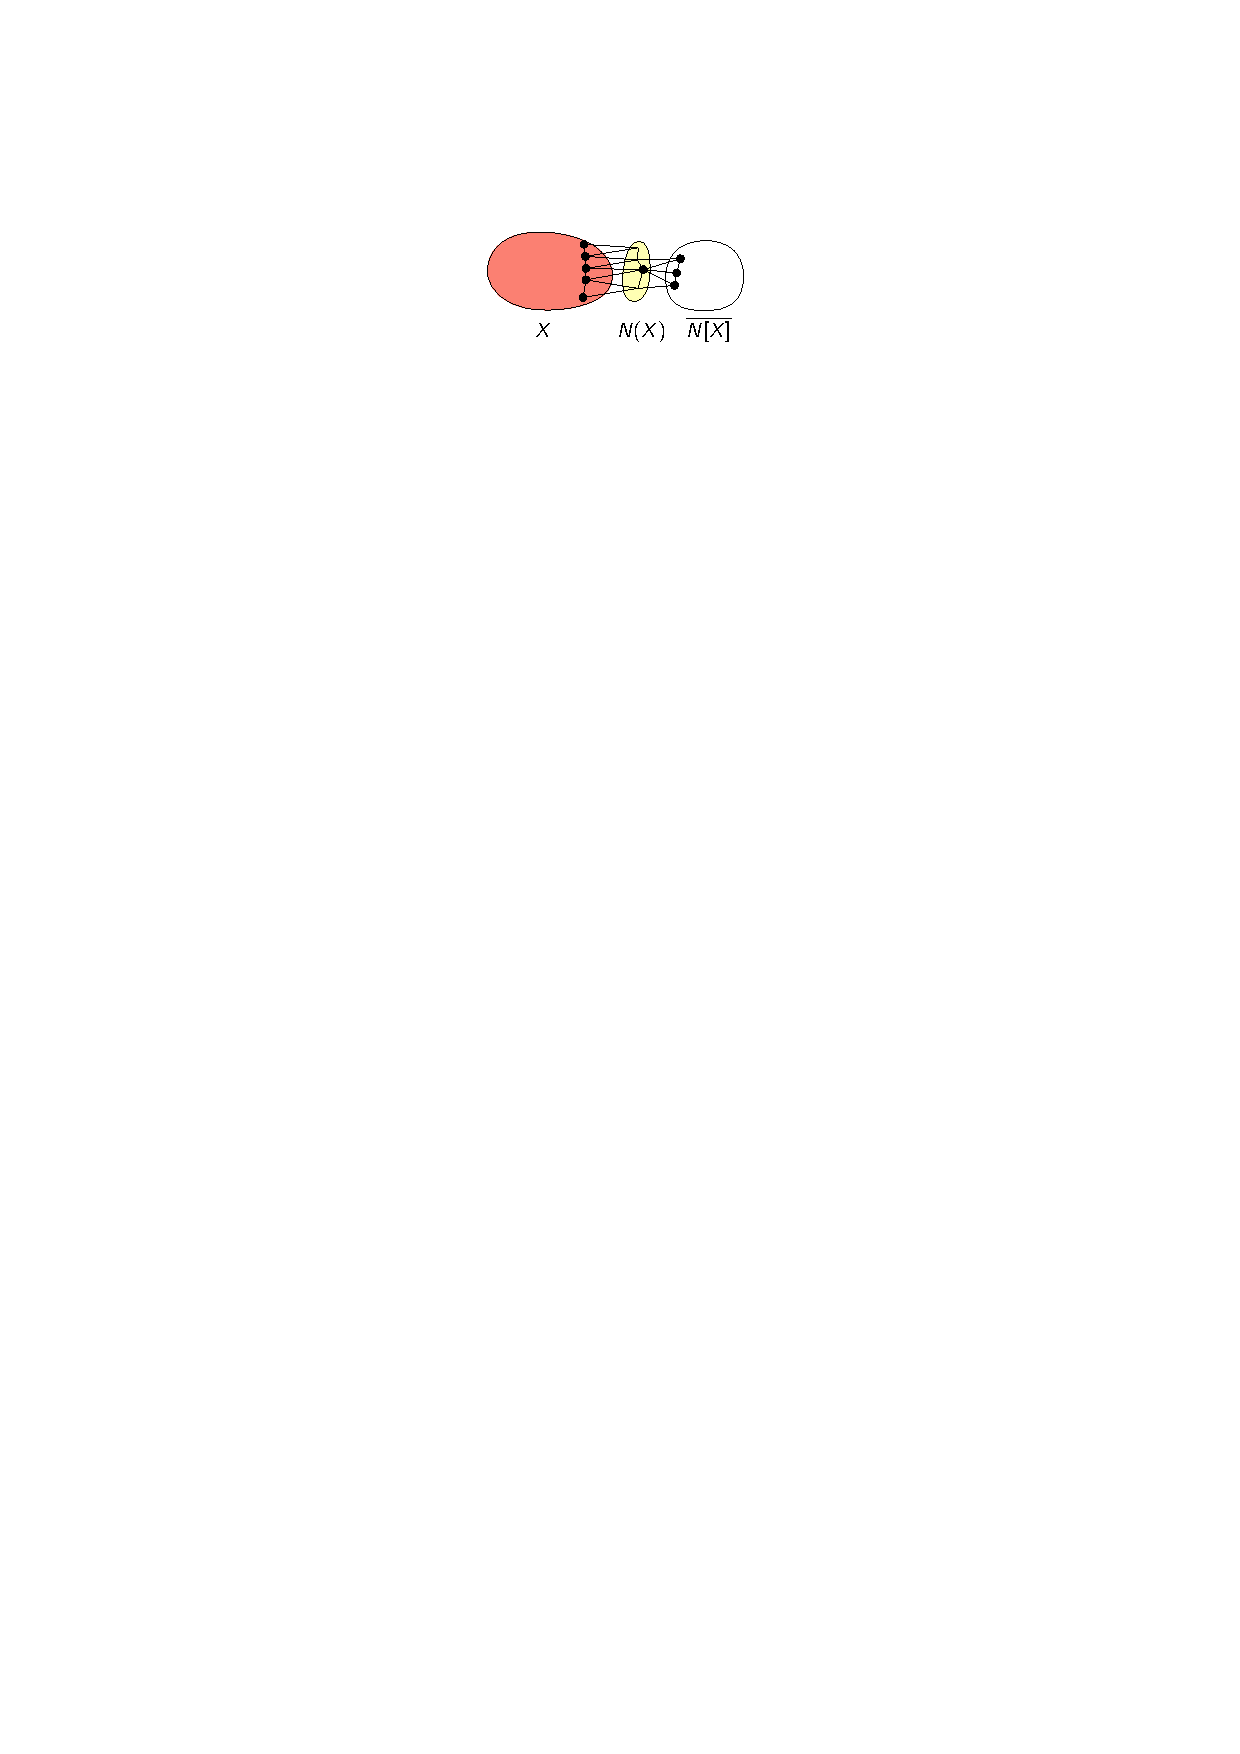
\includegraphics{figs/greedy} \includegraphics[page=6]{figs/walkthrough}
  \end{center}
  \[
     |X| = r + I , \quad 2r + I \le n, \quad I \le (n-r)/4
  \]
  Maximized when $r=3n/7$, $I=n/7$
  }
\end{frame}

\begin{frame}
  \frametitle{Some Lies I've Told}

  \begin{itemize}
    \item Actually a linear program that involves:
    \begin{itemize}
      \item $r$: number of rounds
      \item $x_d$: number of times we choose a vertex of inner-degree $d$
      \item $D$: Number of dominated vertices $\sum_{d\ge 2}d x_d$
      \item $I$: Number of undominated vertices
      \item $B$: Number of \emphh{boundary} vertices  (X---B---I)
    \end{itemize}
    \[
       B \le D - r
    \]
    \[
       D+I \le n
    \]
    \[
      I \le B/3
    \]
    \[
       |X| \le r + I
    \]
  \end{itemize}
\end{frame}

\begin{frame}
  \frametitle{Lessons}

  \begin{itemize}[<+->]
    \item Always taking inner-degree $\ge2$ leads to $|X|\le n/2$
    \item We lose a bit in the final step ($1$-critical graph)
    \item To beat $n/2$, we need to choose vertices of inner-degree $>2$\\[3em]
  \end{itemize}
  \uncover<4->{
  \begin{center}
    But...\\[1em]
    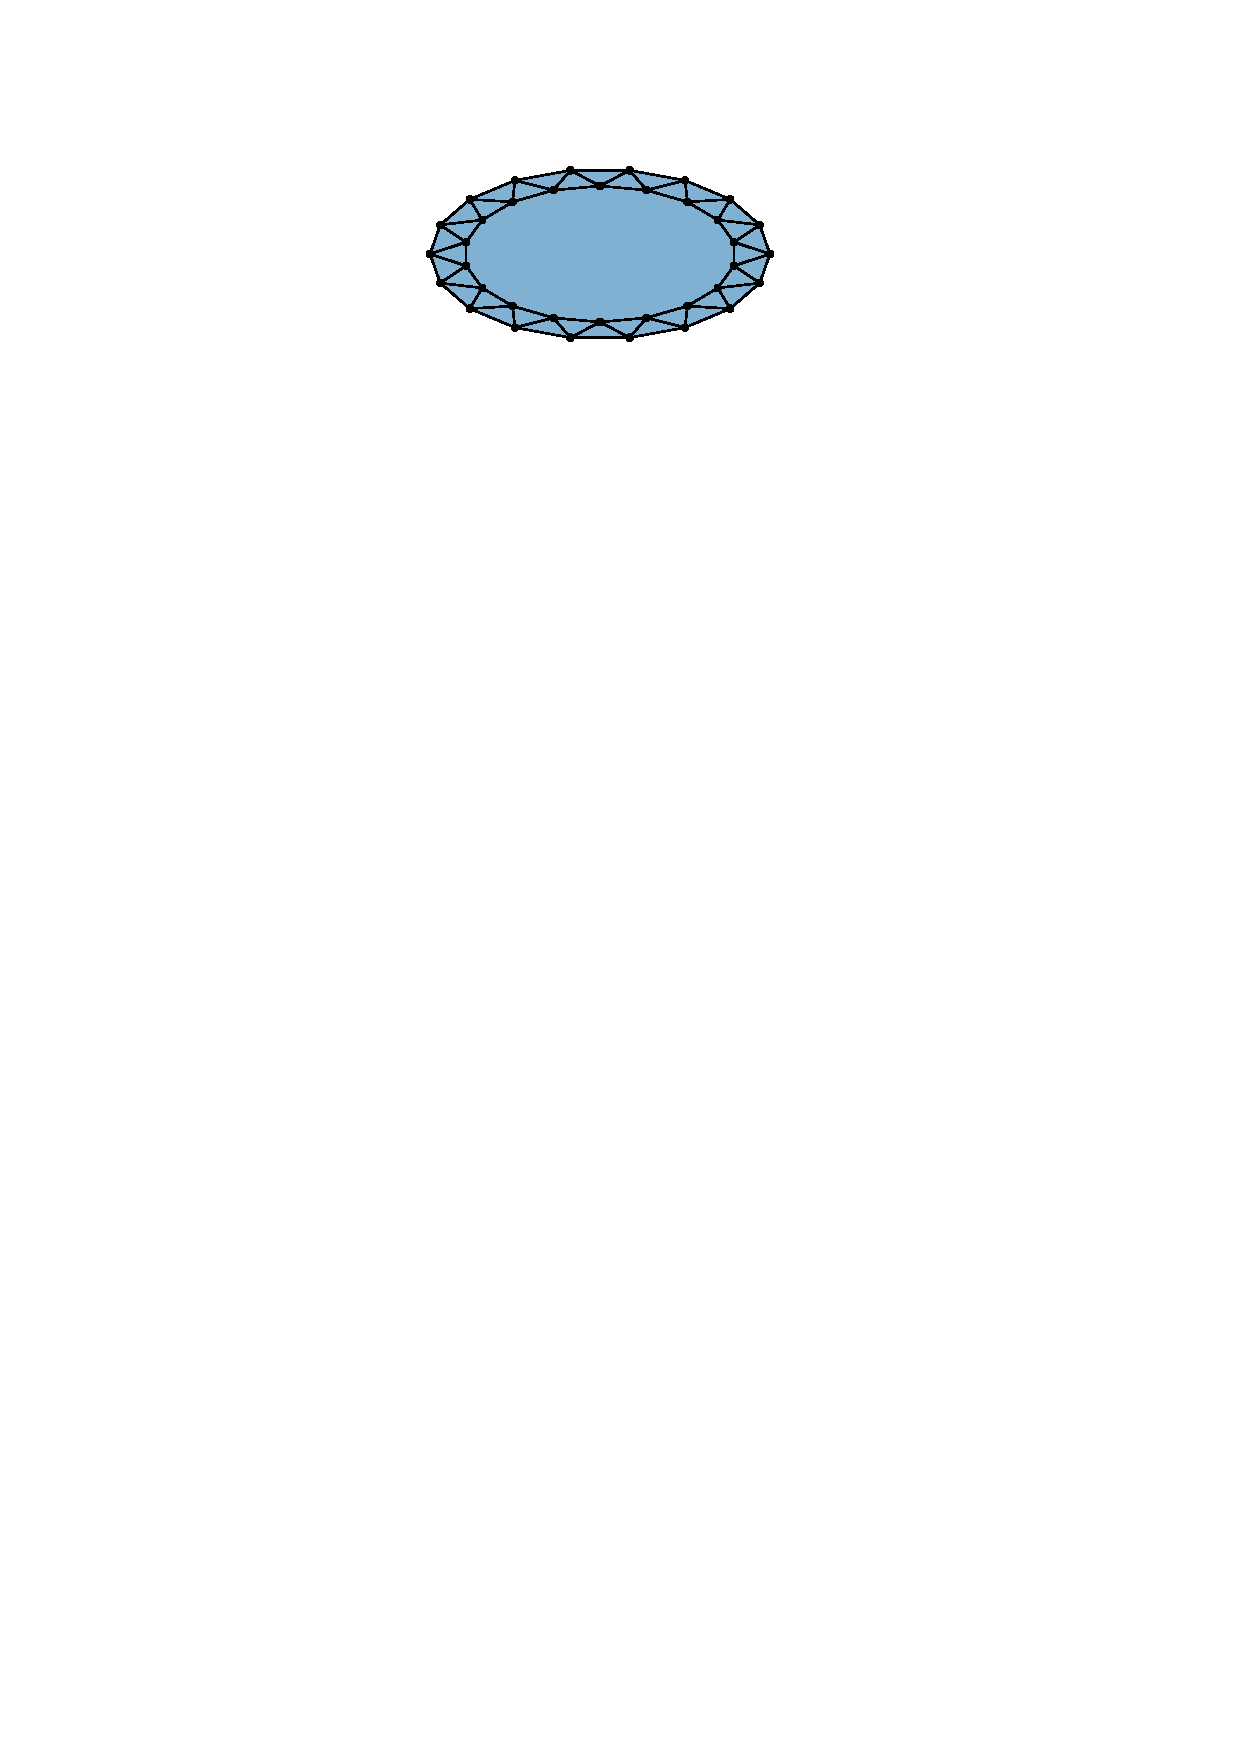
\includegraphics{figs/ring}
  \end{center}
  }
\end{frame}


\begin{frame}
  \frametitle{The Next-Best Thing}

  Take vertices of inner-degree $\ge 2.5$

  \begin{center}
    \only<1>{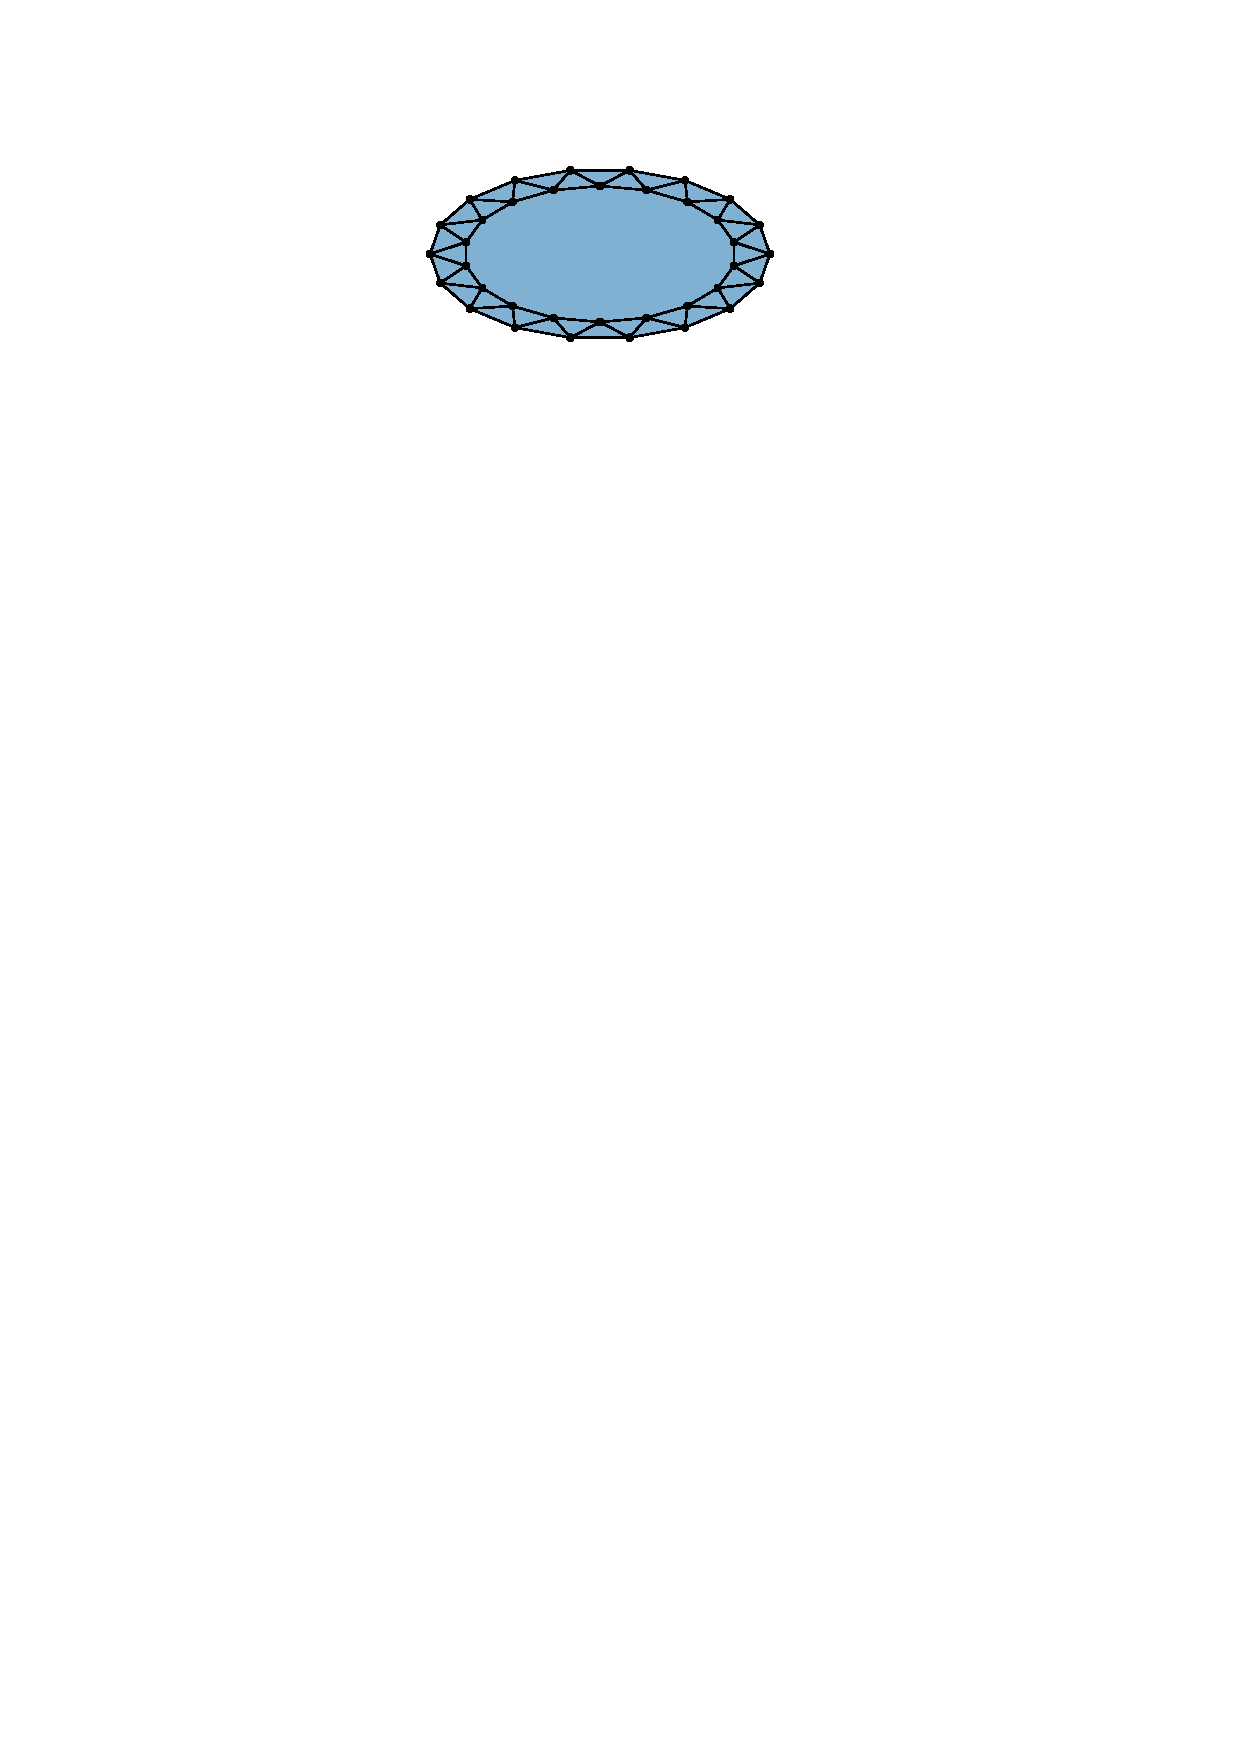
\includegraphics[page=1]{figs/ring}}%
    \only<2>{\includegraphics[page=2]{figs/ring}}%
    \only<3>{\includegraphics[page=3]{figs/ring}}%
    \only<4>{\includegraphics[page=4]{figs/ring}}%
    \only<5>{\includegraphics[page=5]{figs/ring}}%
    \only<6>{\includegraphics[page=6]{figs/ring}}%
    \only<7>{\includegraphics[page=7]{figs/ring}}%
    \only<8-9>{\includegraphics[page=8]{figs/ring}}%
    \only<10->{\includegraphics[page=3]{figs/ring}}%
  \end{center}
  \uncover<9>{Would give $|X|\le n/2.5=2n/5=0.4n$}
\end{frame}


\begin{frame}
  \frametitle{Final Step: $2$-Critical Graphs}

  \begin{center}
    \only<+>{\includegraphics[page=1]{figs/2-critical}}%
    \only<+>{\includegraphics[page=2]{figs/2-critical}}%
    \only<+->{\includegraphics[page=3]{figs/2-critical}}%
    % \only<+>{\includegraphics[page=4]{figs/2-critical}}%
    % \only<+>{\includegraphics[page=5]{figs/2-critical}}%
    % \only<+>{\includegraphics[page=6]{figs/2-critical}}%
    % \only<+>{\includegraphics[page=7]{figs/2-critical}}%
    % \only<+>{\includegraphics[page=8]{figs/2-critical}}%
  \end{center}
  \uncover<4->{
    \[
      \tfrac{2}{3}\operatorname{boundary}(G-N[X]) + \tfrac{1}{3}\operatorname{interior}(G-N[X]) =: \tfrac{2}{3}R + \tfrac{1}{3}S
    \]
  }
\end{frame}

\begin{frame}
  \frametitle{Analysis}

  \textbf{Theorem:} $\textsc{BestGreedy}(G)$ produces a connected dominating set of size at most $10n/21$.\\[1em]

  \textit{Proof:} Takes vertices of inner-degree at least $2.5$ until $G-X$ is $2$-critical then takes $\tfrac{2}{3}R+\tfrac{1}{3}S$ additional vertices

  % \begin{center}
  %   \includegraphics{figs/greedy} \includegraphics[page=6]{figs/walkthrough}
  % \end{center}
  \begin{tabular}{p{.05\textwidth}c}
  \[
     |X| \le r + \tfrac{2}{3}R + \tfrac{1}{3}S
  \]
  \[
     D \ge 2.5r
  \]
  \[
    D + R + S = n
  \]
  \[
    B \le D - r
  \]
  \[
    R \le B
  \]
  \[
    S \le \tfrac{1}{3}R
  \]
  & \raisebox{-\height}{\includegraphics{figs/dbrs}}
  \end{tabular}
  LP gives $|X|\le 10n/21$.
  \uncover<2->{\hfill{$\Box$}}
  % }
\end{frame}

\begin{frame}
  \frametitle{Triangulated Surfaces}

  \textbf{Theorem:} For any $g<n$ every $n$-vertex genus-$g$ triangulated surface has a connected dominating set of size at most $10n/21 + O(\sqrt{gn})$.

  \begin{center}
    \only<1>{\includegraphics[page=1]{figs/slicing}}%
    \only<2>{\includegraphics[page=2]{figs/slicing}}%
    \only<3>{\includegraphics[page=3]{figs/slicing}}%
  \end{center}
\end{frame}

\begin{frame}
  \frametitle{Summary}

    \begin{center}
      mininum connected dominating set ${}\le 10n/21$ \\ \verteq \\
      maximum-leaf spanning tree ${}\ge 11n/21$ \\ \verteq \\
      maximum induced outerplane graph ${}\ge 11n/21$ \\
    \end{center}

\end{frame}


\begin{frame}
  \frametitle{Open problem: Tight bounds}

  For triangulations: Lower Bound is $n/3$ upper bound is $10n/21$.
\end{frame}

% \begin{frame}
%   \frametitle{Open Problem: New approaches}
%
%   Different strategy for SEFENOMAP or one-bend free sets?
%
%   \begin{center}
%     \includegraphics[page=13]{figs/walkthrough} \\
%     \includegraphics[page=8,scale=0.8]{figs/proper_good}
%   \end{center}
% \end{frame}
%
% \begin{frame}
%   \frametitle{Open Problem: One-Bend SEFENOMAP}
%
%   SEFENOMAP where all edges of $G_1$ have small complexity?
%
%   \begin{center}
%     \begin{tabular}{cc}
%     \includegraphics[page=1,scale=.8]{figs/sefenomap} & \includegraphics[page=2,scale=.8]{figs/sefenomap} \\
%     $G_1$ & $G_2$
%   \end{tabular}
%   \end{center}
% \end{frame}
%
% \begin{frame}
%   \frametitle{Open Problem: CDS in edge-maximal beyond-planar classes}
%
%     Connected dominating sets in edge-maximal beyond-planar classes? \\[2em]
%
%     For edge-maximal $1$-planar, lower bound is also $n/3$
%     \begin{center}
%       \includegraphics[page=2,scale=1.5]{figs/nover3}
%     \end{center}
%
% \end{frame}

\begin{frame}

  \resizebox{\textwidth}{!}{Thank You!}

\end{frame}

\end{document}
